\documentclass[article]{jss}

\usepackage[utf8]{inputenc}
\usepackage{tikz}
\usepackage{natbib}

%%%%%%%%%%%%%%%%%%%%%%%%%%%%%%
%% declarations for jss.cls %%%%%%%%%%%%%%%%%%%%%%%%%%%%%%%%%%%%%%%%%%
%%%%%%%%%%%%%%%%%%%%%%%%%%%%%%

%% almost as usual
\author{		Michael C. Sachs\\Biometric Research Branch, Division of Cancer Treatment and Diagnosis,
National Cancer Institute		}

\title{\pkg{plotROC}: A Better Tool for Plotting ROC Curves}

%% for pretty printing and a nice hypersummary also set:
\Plainauthor{ Michael C. Sachs} %% comma-separated
\Plaintitle{plotROC: A Better Tool for Plotting ROC Curves} %% without formatting

\Shorttitle{\pkg{plotROC}: A Better Tool for Plotting ROC Curves} %% a short title (if necessary)
%% an abstract and keywords
\Abstract{
  Plots of the receiver operating characteristic (ROC) curve are
  ubiquitous in medical research. Designed to simultaneously display the
  operating characteristics at every possible value of a continuous
  diagnostic test, ROC curves are used in oncology to evaluate screening,
  diagnostic, prognostic and predictive biomarkers. I reviewed a sample of
  ROC curve plots from the major oncology journals in order to assess
  current trends in usage and design elements. My review suggests that ROC
  curve plots are often ineffective as statistical charts and that poor
  design obscures the relevant information the chart is intended to
  display. I describe my new \proglang{R} package that was created to
  address the shortcomings of existing tools. The package has functions to
  create informative ROC curve plots, with sensible defaults, for use in
  print or as an interactive web-based plot. A web application was
  developed to reach a broader audience of scientists who do not use R.
}
\Keywords{ROC curves; graphics; interactive; plots}
\Plainkeywords{ROC curves; graphics; interactive; plots} %% without formatting
%% at least one keyword must be supplied

%% publication information
%% NOTE: Typically, this can be left commented and will be filled out by the technical editor
%% \Volume{50}
%% \Issue{9}
%% \Month{June}
%% \Year{2012}
%% \Submitdate{2012-06-04}
%% \Acceptdate{2012-06-04}

%% The address of (at least) one author should be given
%% in the following format:
\Address{
    Michael C. Sachs\\
    9609 Medical Center Drive, MSC 9735\\
    Bethesda, MD 20892\\
    telephone: 240-276-7888  \\\email{michael.sachs@nih.gov}
}
%% It is also possible to add a telephone and fax number
%% before the e-mail in the following format:
%% Telephone: +43/512/507-7103
%% Fax: +43/512/507-2851

%% for those who use Sweave please include the following line (with % symbols):
%% need no \usepackage{Sweave.sty}

%% end of declarations %%%%%%%%%%%%%%%%%%%%%%%%%%%%%%%%%%%%%%%%%%%%%%%


\begin{document}

\section{Introduction}\label{introduction}

\subsection{About ROC Curves}\label{about-roc-curves}

The Receiver Operating Characteristic (ROC) curve is used to assess the
accuracy of a continuous measurement for predicting a binary outcome. In
medicine, ROC curves have a long history of use for evaluating
diagnostic tests in radiology and general diagnostics. ROC curves have
also been used for decades in signal detection theory.

The accuracy of a diagnostic test can be evaluated by considering two
possible types of errors: false positives, and false negatives. For a
continuous measurement that I denote as \(M\), convention dictates that
a test positive is defined as \(M\) exceeding some fixed threshold
\(c\): \(M > c\). In reference to the binary outcome that I denote as
\(D\), a good outcome of the test is when the test is positive for an
individual who truly has a disease: \(D = 1\). A bad outcome is when the
test is positive for an individual who does not have the disease
\(D = 0\).

Formally, for a fixed cutoff \(c\), the true positive fraction is the
probability of a test positive in the diseased population:

\[ TPF(c) = P\{ M > c | D = 1 \} \]

and the false positive fraction is the probability of a test positive in
the healthy population:

\[ FPF(c) = P\{ M > c | D = 0 \} \]

Since the cutoff \(c\) is not fixed in advance, I can plot the TPF
against the FPF for all possible values of \(c\). This is exactly what
the ROC curve is, a plot of \(FPF(c)\) on the \(x\) axis and \(TPF(c)\)
along the \(y\) axis as \(c\) varies. A useless test that is not
informative at all in regards to the disease status has
\(TPF(c) = FPF(c)\) for all \(c\). The ROC plot of a useless test is
thus the diagonal line. A perfect test that is completely informative
about disease status has \(TPF(c) = 1\) and \(FPF(c) = 0\) for all
\(c\).

Given a sample of test and disease status pairs,
\((M_1, D_1), \ldots, (M_n, D_n)\), I can estimate the ROC curve by
computing proportions in the diseased and healthy subgroups separately.
Specifically, given a fixed cutoff \(c\), an estimate of the \(TPF(c)\)
is

\[ \widehat{TPF(c)} = \frac{\sum_{i = 1}^n 1\{M_i > c\} \cdot 1\{D_i = 1\}}{\sum_{i=1}^n 1\{D_i = 1\}}, \]

where \(1\{\cdot\}\) is the indicator function. An estimate for
\(FPF(c)\) is given by a similar expression with \(D_i = 1\) replaced
with \(D_i = 0\). Calculating these proportions for \(c\) equal to each
unique value of the observed \(M_i\) yields what is known as the
empirical ROC curve estimate. The empirical estimate is a step function.
Other methods exist to estimate the ROC curve, such as the binormal
parametric estimate which can be used to get a smooth curve. There are
also extensions that allow for estimation with time-to-event outcomes
subject to censoring. For a more thorough reference on the methods and
theory surrounding ROC curves, I refer interested readers to
\citet{pepe2003statistical}.

A common way to summarize the value of a test for classifying disease
status is to calculate the area under the ROC curve (AUC). The greater
the AUC, the more informative the test. The AUC summarizes the
complexities of the ROC curve into a single number and therefore is
widely used to facilitate comparisons between tests and across
populations. It has been criticized for the same reason because it does
not fully characterize the trade-offs between false- and true-positives.

\subsection{Design Considerations}\label{design-considerations}

The main purpose of visually displaying the ROC curve is to show the
trade-off between the FPF and TPF as the cutoff \(c\) varies. This can
be useful for aiding viewers in choosing an optimal cutoff for decision
making, for comparing a small number of candidate tests, and for
generally illustrating the performance of the test as a classifier. In
practice, once the FPF and TPF are computed for each unique observed
cutoff value, they can be plotted as a simple line chart or scatter plot
using standard plotting tools. This often leads to the unfortunate
design choice of obscuring the critical and useful third dimension, the
range of cutoff values \(c\).

Another key design element is the use of a diagonal guideline for
comparison. They allow observers to roughly estimate the area between
the diagonal and the estimated ROC curve, which serves as a proxy for
estimating the value of the test for classification above a useless
test. Likewise, gridlines inside the plotting region and carefully
selected axes allow for accurate assessment of the TPF and FPF at
particular points along the ROC curve. Many medical studies use ROC
curves to compare a multitude of candidate tests to each other. In those
cases, curves need to be distinguished by using different colors or line
types combined with a legend, or direct labels inside the plotting
region.

In the medical literature, FPF and TPF are usually referred to in terms
of the jargon sensitivity and specificity. Sensitivity is equivalent to
the true positive fraction. Specificity is 1 - FPF, the true negative
fraction. Sometimes, the FPF and TPF are incorrectly referred to as
rates, using the abbreviations FPR and TPR. These are probabilities and
their estimates are proportions, therefore I prefer the use of the term
fraction as opposed to rate.

\subsection{Existing Plotting
Software}\label{existing-plotting-software}

The ROC curve plot is, at the most basic level, a line graph. Therefore,
once the appropriate statistics are estimated, existing plotting
functions can be used to create an ROC curve plot. Viewers can identify
ROC plots through context, by observing the shape of the line, and
through the addition of axis labels, titles, legends, and so on. In my
review of the oncology literature, I observed plots with the distinctive
characteristics of the plotting functions from Microsoft Office,
\proglang{SAS}, \proglang{SPSS}, and the base \proglang{R} plotting
functions \citep{arr}.

There are several \proglang{R} packages related to ROC curve estimation
that contain dedicated plotting functions. The \pkg{ROCR} package
\citep{rocr} plots the FPF \emph{versus} TPF, as usual, and then takes
the interesting approach of encoding the cutoff values as a separate
color scale along the ROC curve itself. A legend for the color scale is
placed along the vertical axis on the right of the plotting region. The
\pkg{pROC} package \citep{pROC} is mainly focused on estimating
confidence intervals and regions for restricted ranges of the ROC curve.
The plotting methods therein use the base \proglang{R} plotting
functions to create nice displays of the curves along with shaded
confidence regions. My \pkg{plotROC} package uses the \pkg{ggplot2}
\citep{ggplot2} plotting library to create clear, informative ROC plots,
with interactive features for use on the web, and sensible defaults for
use in print.

\subsection{Motivation}\label{motivation}

Anyone giving a cursory look at any of the major medical journals is
likely to find at least one ROC curve plot. I sought to assess the usage
of ROC curve plots and to evaluate the design choices made in the
current oncology literature by conducting a small literature review. I
searched Pubmed for clinical trials or observational studies in humans
reported in major oncology journals for the past 10 years for the terms
``ROC Curve'' OR ``ROC Analysis'' OR ``Receiver operating characteristic
curve''. The search was conducted on October 8, 2014 and returned 54
papers. From those papers, 47 images were extracted and reviewed. The
exact specifications for the Pubmed query are available in the
manuscript source files.

Each image consisted of a single ROC curve plot or a panel of multiple
plots. Each plot was inspected manually for the following design
features: the number of curves displayed, the type of axis labels
(sensitivity/ 1 - specificity or true/false positive fractions),
presence or absence of grid lines, presence or absence of a diagonal
guide line, whether any cutpoints were indicated, the type of curve
label (legend or direct label), and presence of other textual
annotations such as the AUC. The numerical results of the survey are
summarized in table \ref{table1}.

\begin{table}[ht]
\centering
\begin{tabular}{ll}
  \hline
 & percent (count) \\ 
  \hline
Number of curves &  \\ 
  $\quad$1 & 19.6 (9) \\ 
  $\quad$2 & 43.5 (20) \\ 
  $\quad$3 & 10.9 (5) \\ 
  $\quad$4+ & 26.1 (12) \\ 
  $\quad$Average (SD) & 2.6 (1.5) \\ 
  Axis labels &  \\ 
  $\quad$FPF/TPF & 13.0 (6) \\ 
  $\quad$mixed & 2.2 (1) \\ 
  $\quad$none & 2.2 (1) \\ 
  $\quad$sens/spec & 82.6 (38) \\ 
  Diagonal Guide & 43.5 (20) \\ 
  Gridlines & 17.4 (8) \\ 
  Cutoffs indicated & 15.2 (7) \\ 
  AUC indicated & 50.0 (23) \\ 
  Curve Labels &  \\ 
  $\quad$direct & 10.9 (5) \\ 
  $\quad$legend & 63.0 (29) \\ 
  $\quad$none & 19.6 (9) \\ 
  $\quad$title & 6.5 (3) \\ 
   \hline
\end{tabular}
\caption{Results of a literature review of major oncology journals for ROC curve plots. The rows indicate the frequency and count of key design elements of an ROC curve plot. FPR = False positive rate; TPR = True positive rate; sens = Sensitivity; spec = Specificity; AUC = Area under the Curve} 
\label{table1}
\end{table}

The small minority of the figures make any attempt to indicate the
values of the test cutoffs, which is an integral component of the ROC
curve. I conjecture that this is mainly due to the use of default
plotting procedures in statistical software. The software, by default,
treats the ROC curve as a 2 dimensional object, obscuring the cutoff
dimension. Gridlines and direct labels are also somewhat out of the
ordinary. The absence of these features make accurate determination and
comparison of the values more difficult. Many of the plots included
large tables containing estimates and inference for AUCs, while the ROC
curves themselves, numerous and without clear labels or reference lines,
merely served as decoration. I aim to solve some of these problems by
providing an easy-to-use plotting interface for the ROC curve that
provides sensible defaults.

The panels of figure \ref{figure1} illustrate the most common styles of
ROC curve plots, and the associated design elements. I favor the use of
gridlines and a diagonal reference line to facilitate accurate readings
off of the axes. Direct labels are preferred over legends because they
omit the additional cognitive step of matching line types or colors to
labels. My \pkg{plotROC} package additionally provides plotting of
cutoff values, which are displayed interactively with the web-based
output option, and direct labels for print use. Exact confidence regions
for points on the ROC curve are optionally calculated and displayed.
Additionally, I use axis scales adjusted to be denser near the margins 0
and 1. In medical applications, it is often necessary to have a very low
FPR (less than 10\%, for instance), therefore the smaller scales are
useful for accurately determining values near the margins. The next
section details the usage of the \pkg{plotROC} \proglang{R} package and
these features.

\begin{figure}[htbp]
\centering
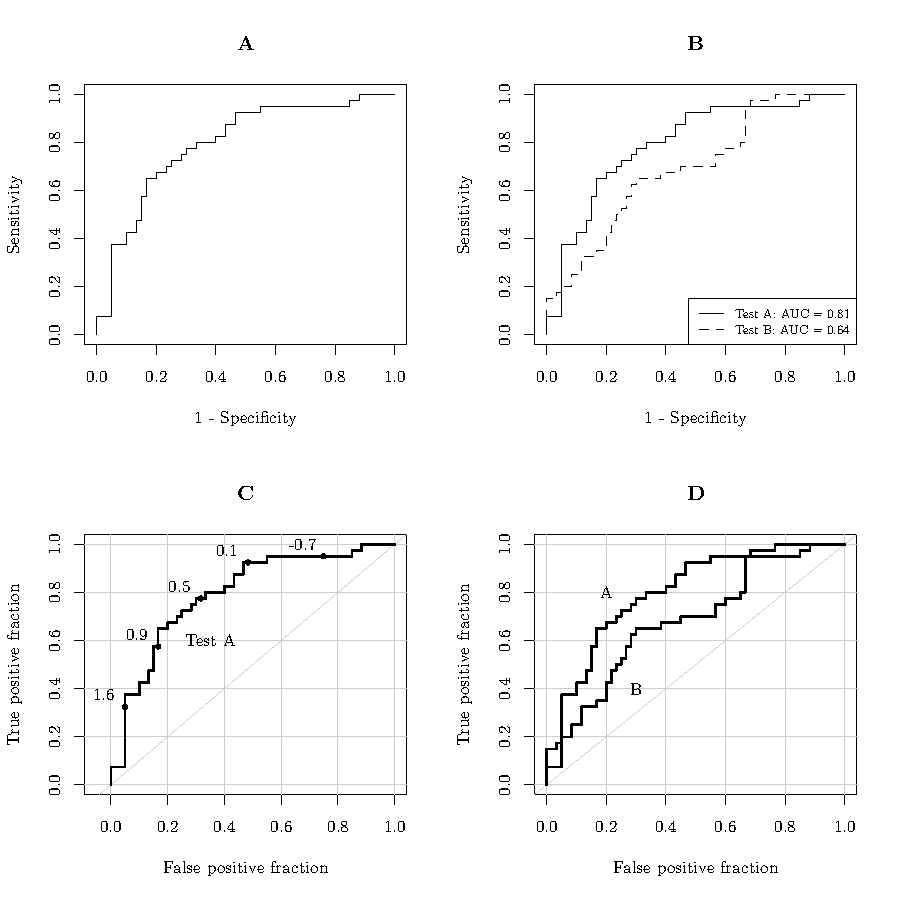
\includegraphics{figure/figure1-1.pdf}
\caption{Illustration of design choices in plotting ROC curves. Panel A
shows a sparse ROC curve, with no design additions inside the plotting
region. The plot results in more white space than anything else. It is
difficult to accurately determine values without reference lines. Panel
B shows a plot comparing 2 curves, with different line types and a
legend. AUCs are also given in the legend. Panels B and C add gridlines,
diagonal reference lines, and direct labels. \label{figure1}}
\end{figure}

\section{Usage of the Package}\label{usage-of-the-package}

\subsection{Shiny application}\label{shiny-application}

I created a \pkg{shiny} application \citep{shiny} in order to make the
features more accessible to non-\proglang{R} users. A limited subset of
the functions of \pkg{plotROC} can be performed on an example dataset or
on data that users upload to the website. Resulting plots can be saved
to the users' machine as a pdf or as a stand-alone html file. It can be
used in any modern web browser with no other dependencies at the website
here: http://sachsmc.shinyapps.io/plotROC.

\subsection{Installation and loading}\label{installation-and-loading}

\pkg{plotROC} can be installed from the Comprehensive \proglang{R}
Archive Network, or installed from source.

\begin{verbatim}
install.packages("plotROC")
library(plotROC)
\end{verbatim}

\subsection{Quick start}\label{quick-start}

After installing, the interactive Shiny application can be run locally.

\begin{verbatim}
shiny_plotROC()
\end{verbatim}

\subsection{Command line basic usage}\label{command-line-basic-usage}

I start by creating an example data set. The marker I generate is
moderately accurate for predicting disease status.

\begin{verbatim}
D.ex <- rbinom(100, size = 1, prob = .5)
M.ex <- rnorm(100, mean = D.ex)
\end{verbatim}

Next I use the \texttt{calculate\_roc} function to compute the empirical
ROC curve. The disease status need not be coded as 0/1, but if it is
not, \texttt{calculate\_roc} assumes (with a warning) that the lowest
value in sort order signifies disease-free status. This returns a
dataframe with three columns: the cutoff values, the TPF and the FPF.

\begin{verbatim}
roc.estimate <- calculate_roc(M.ex, D.ex)
str(roc.estimate)
\end{verbatim}

\begin{verbatim}
'data.frame':   100 obs. of  3 variables:
 $ c  : num  -2.18 -1.67 -1.57 -1.55 -1.54 ...
 $ TPF: num  1 1 1 1 1 1 1 1 1 1 ...
 $ FPF: num  0.981 0.962 0.943 0.925 0.906 ...
\end{verbatim}

The \texttt{rocdata} is passed to the \texttt{ggroc} function with an
optional label. This creates a ggplot object of the ROC curve using the
\pkg{ggplot2} package \citep{ggplot2}.

\begin{verbatim}
single.rocplot <- ggroc(roc.estimate, label = "Example")
\end{verbatim}

The \texttt{myrocplot} object can be used to create an interactive plot
and display it in the Rstudio viewer or default web browser by passing
it to the \texttt{plot\_interactive\_roc} function. Give the function an
optional path to an html file as an argument called \texttt{file} to
save the interactive plot as a complete web page. A screen shot of an
interactive plot is shown in figure \ref{interact}. Hovering over the
display shows the cutoff value at the point nearest to the cursor.
Clicking makes the cutoff label stick until the next click, and if
confidence regions are available, clicks will also display those as grey
rectangles.

\begin{verbatim}
plot_interactive_roc(single.rocplot)
\end{verbatim}

\begin{figure}[ht]
\centering
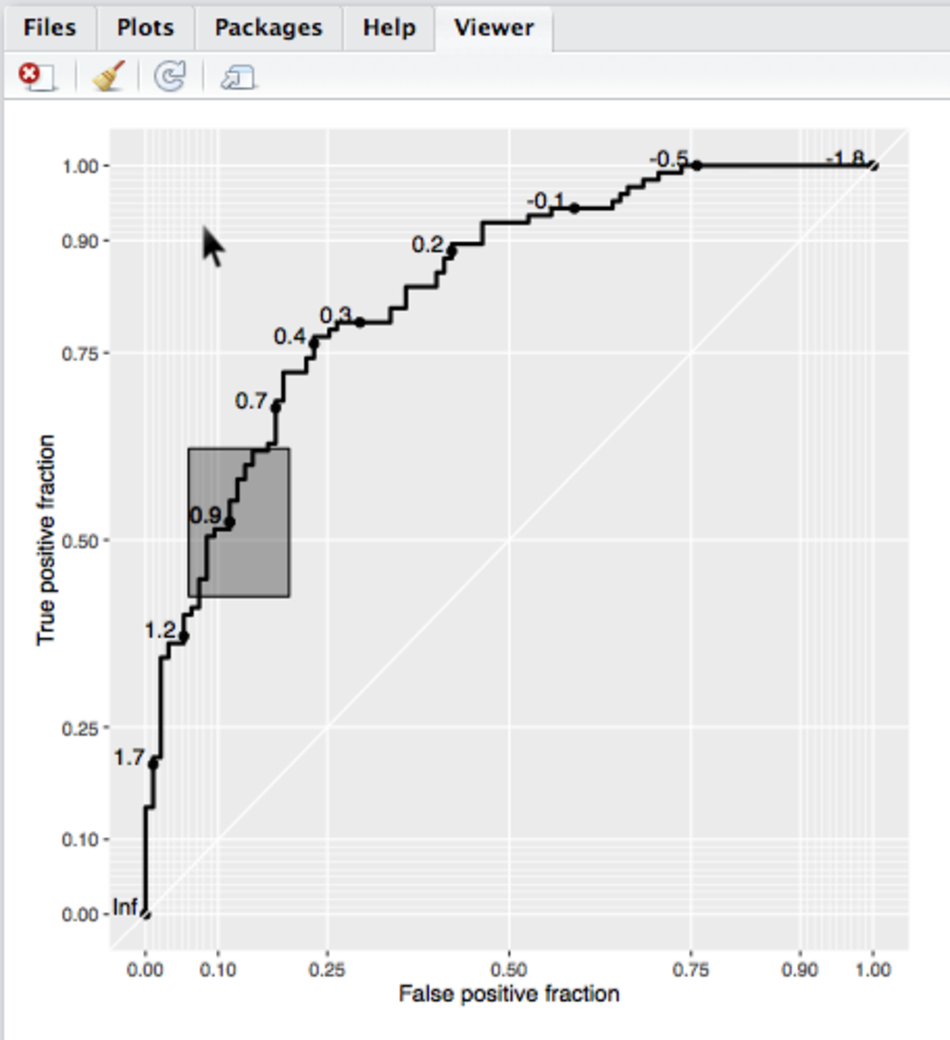
\includegraphics{figure/screen-shot.pdf}
\caption{Screen shot of an interactive plot created with \pkg{plotROC} being displayed in the Rstudio viewer. Hovering the mouse cursor over the plot causes the cutoff label nearest to the cursor to be displayed. Clicking will display a confidence region, if available, and make the label stick until the next click. For live examples, see the package vignette, or go to http://sachsmc.github.io/plotROC. \label{interact}}
\end{figure}

An interactive ROC plot can be exported by using the
\texttt{export\_interactive\_roc} function, which returns a character
string containing the necessary \proglang{HTML} and
\proglang{JavaScript}. The character string can be copy-pasted into an
html document, or better yet, incorporated directly into a dynamic
document using \pkg{knitr} \citep{knitr}. In a \pkg{knitr} document, it
is necessary to use the \texttt{cat} function on the results and use the
chunk option \texttt{results = \textquotesingle{}asis\textquotesingle{}}
so that the interactive plot is displayed correctly. For documents that
contain multiple interactive plots, it is necessary to assign each plot
a unique name using the \texttt{prefix} argument of
\texttt{export\_interactive\_roc}. This is necessary to ensure that the
\proglang{JavaScript} code manipulates the correct svg elements. For
examples of interactive plots and how to incorporate them into
\pkg{knitr} documents, see the package vignette
(\texttt{vignette("examples", package = "plotROC")}) or the web page
https://sachsmc.github.io/plotROC/. The next code block shows an example
\pkg{knitr} chunk that can be used in an .Rmd document to display an
interactive plot.

\begin{verbatim}
```{r int-no, results = 'asis'}
cat(
  export_interactive_roc(single.rocplot, 
                        prefix = "a")
  )
```
\end{verbatim}

The same \texttt{ggroc} object that I called \texttt{myrocplot} can be
used to generate an ROC plot suitable for use in print. It annotates the
cutoff values and is completely in black and white. A simple example
with the default options is shown in figure \ref{first}.

\begin{verbatim}
plot_journal_roc(single.rocplot)
\end{verbatim}

\begin{figure}[htbp]
\centering
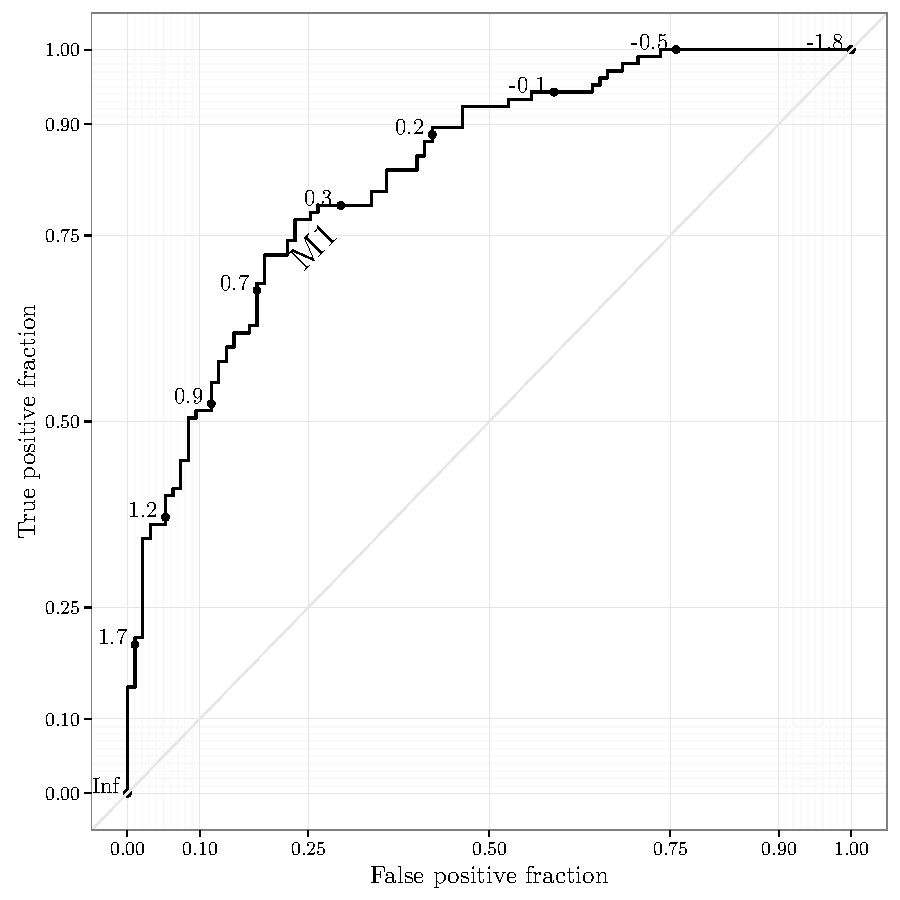
\includegraphics{figure/print-1.pdf}
\caption{Illustration of ROC curve plot generated by \pkg{plotROC} for
use in print. \label{first}}
\end{figure}

\subsubsection{Multiple ROC curves}\label{multiple-roc-curves}

If you have multiple tests of different types measured on the same
subjects, you can use the \texttt{calculate\_multi\_roc} function to
compute the empirical ROC curve for each test. It returns a list of data
frames with the estimates and cutoff values. Then the
\texttt{multi\_ggroc} function creates the appropriate type of
\texttt{ggplot} object. Confidence regions are not supported for
multiple curves at the time of writing.

\begin{verbatim}
D.ex <- rbinom(100, 1, .5)

paired.data <- data.frame(M1 = rnorm(100, mean = D.ex), 
                       M2 = rnorm(100, mean = D.ex, sd = .4), 
                       M3 = runif(100), D = D.ex)

estimate.list <- calculate_multi_roc(paired.data, c("M1", "M2", "M3"), "D")
\end{verbatim}

Labels can be added easily with the \texttt{label} option of
\texttt{multi\_ggroc}. The length of the label element should match the
number of plotted curves. The \texttt{multi\_ggroc} object can be passed
to the \texttt{plot\_journal\_roc} and the
\texttt{export\_interactive\_roc} functions, as desired. The resulting
plot is shown in figure \ref{multi}.

\begin{verbatim}
multi.rocplot <- multi_ggroc(estimate.list, label = c("M1", "M2", "M3"))
plot_journal_roc(multi.rocplot)
\end{verbatim}

\begin{figure}[htbp]
\centering
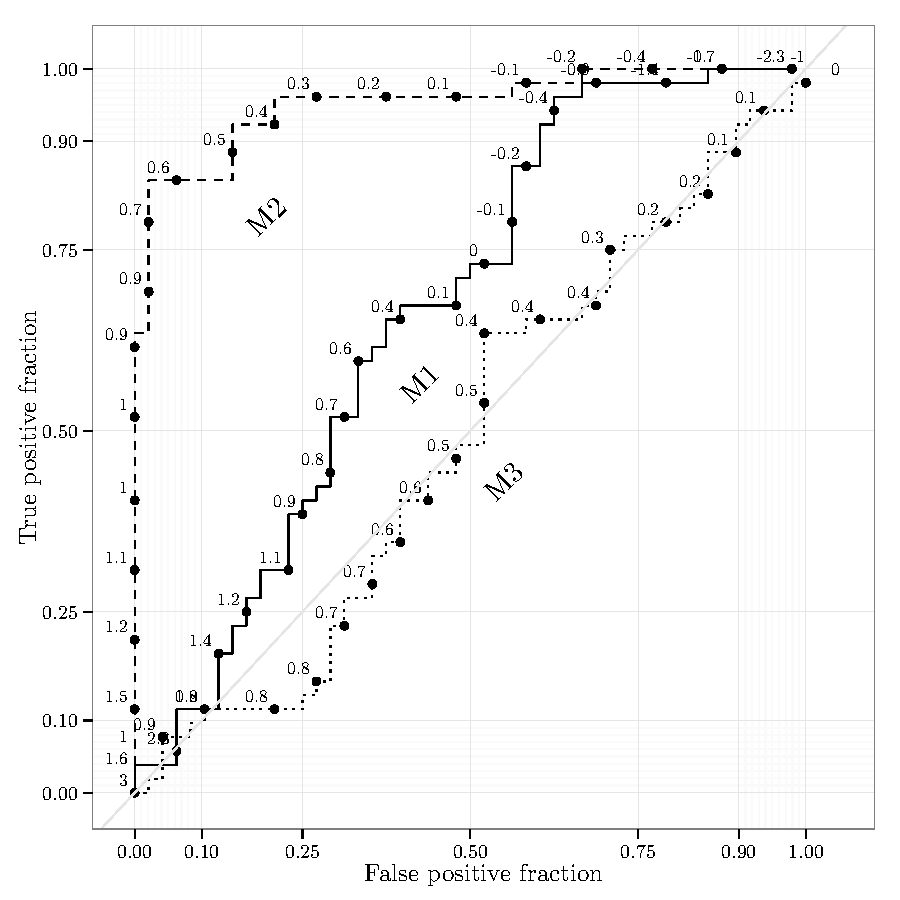
\includegraphics{figure/multi2-1.pdf}
\caption{Illustration of \pkg{plotROC} plot with multiple curves.
\label{multi}}
\end{figure}

Both \texttt{plot\_journal\_roc} and \texttt{export\_interactive\_roc}
support a number of options to customize the look of the plots. By
default, multiple curves are distinguished by different line types and
direct labels. For multiple ROC curves that are similar to one another,
those defaults can make it difficult to interpret the plots. Therefore,
we also support colors and legends. The x- and y-axis can be changed by
passing options to \texttt{ggroc} or \texttt{multi\_ggroc}. The next
code block illustrates the available options.

\begin{verbatim}
colorplot <- multi_ggroc(estimate.list, 
                         xlabel = "1 - Specificity", 
                         ylabel = "Sensitivity")
cat(
  export_interactive_roc(colorplot, lty = rep(1, 3), 
                         color = c("black", "purple", "orange"), 
                         legend = TRUE)
  )
\end{verbatim}

\subsection{Advanced options}\label{advanced-options}

\subsubsection{Click to view confidence
region}\label{click-to-view-confidence-region}

I use the \texttt{ci = TRUE} option in \texttt{calculcate\_roc} and
\texttt{ggroc} to compute confidence regions for points on the ROC curve
using the \citet{clopper1934use} exact method. Briefly, exact confidence
intervals are calculated for the \(FPF\) and \(TPF\) separately, each at
level \(1 - \sqrt{1 - \alpha}\). Based on result 2.4 from
\citet{pepe2003statistical}, the cross-product of these intervals yields
a \(100 * (1 - \alpha)\) percent rectangular confidence region for the
pair. The significance level can be specified using the \texttt{alpha}
option.

\begin{verbatim}
roc.ci <- calculate_roc(paired.data$M1, paired.data$D, ci = TRUE, alpha = 0.05)
ci.rocplot <- ggroc(roc.ci, label = "CI Example", ci = TRUE)
\end{verbatim}

For interactive plots, the confidence regions are automatically
detected. When the user clicks on the ROC curve, the confidence region
for the TPF and FPF is overlaid using a grey rectangle. The label and
region stick until the next click.

\begin{verbatim}
cat(
  export_interactive_roc(ci.rocplot, 
                         prefix = "aci")
  )
\end{verbatim}

For use in print, I pass a small vector of cutoff locations at which to
display the confidence regions. This is shown in figure \ref{conf}.

\begin{verbatim}
plot_journal_roc(ci.rocplot, n.cuts = 10, 
                 ci.at = c(-.5, .5, 2.1))
\end{verbatim}

\begin{figure}[htbp]
\centering
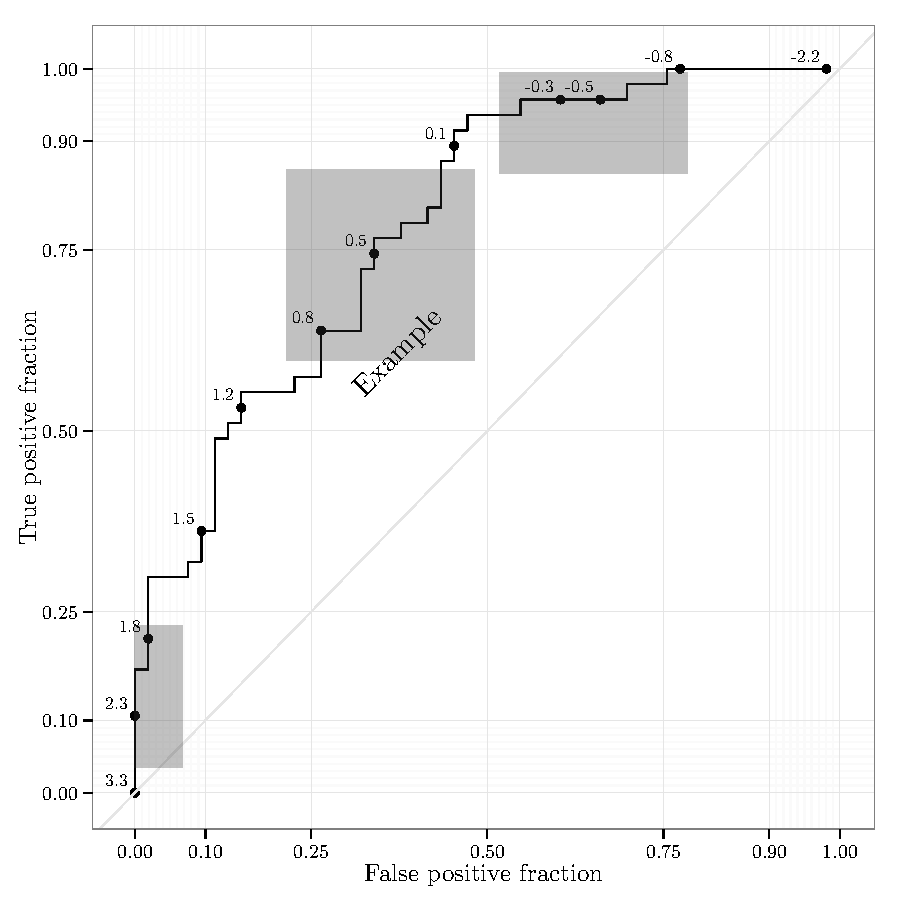
\includegraphics{figure/printci-1.pdf}
\caption{Illustration of \pkg{plotROC} plot with exact confidence
regions. \label{conf}}
\end{figure}

\subsubsection{Themes and annotations}\label{themes-and-annotations}

\pkg{plotROC} uses the \pkg{ggplot2} package to create the objects to be
plotted. Therefore, themes and annotations can be added in the usual
\pkg{ggplot2} way. A \texttt{plot\_journal\_roc} figure with a new
theme, title, axis label, and AUC annotation is shown in figure
\ref{annotate}.

\begin{verbatim}
library(ggplot2)
plot_journal_roc(ci.rocplot, n.cuts = 10, 
                 ci.at = c(-.5, .5, 2.1)) + 
  theme_grey() + 
  geom_abline(intercept = 0, slope = 1, color = "white") + 
  ggtitle("Themes and annotations") + 
  annotate("text", x = .75, y = .25, 
           label = "AUC = 0.80") +
  scale_x_continuous("1 - Specificity", breaks = seq(0, 1, by = .1))
\end{verbatim}

\begin{figure}[htbp]
\centering
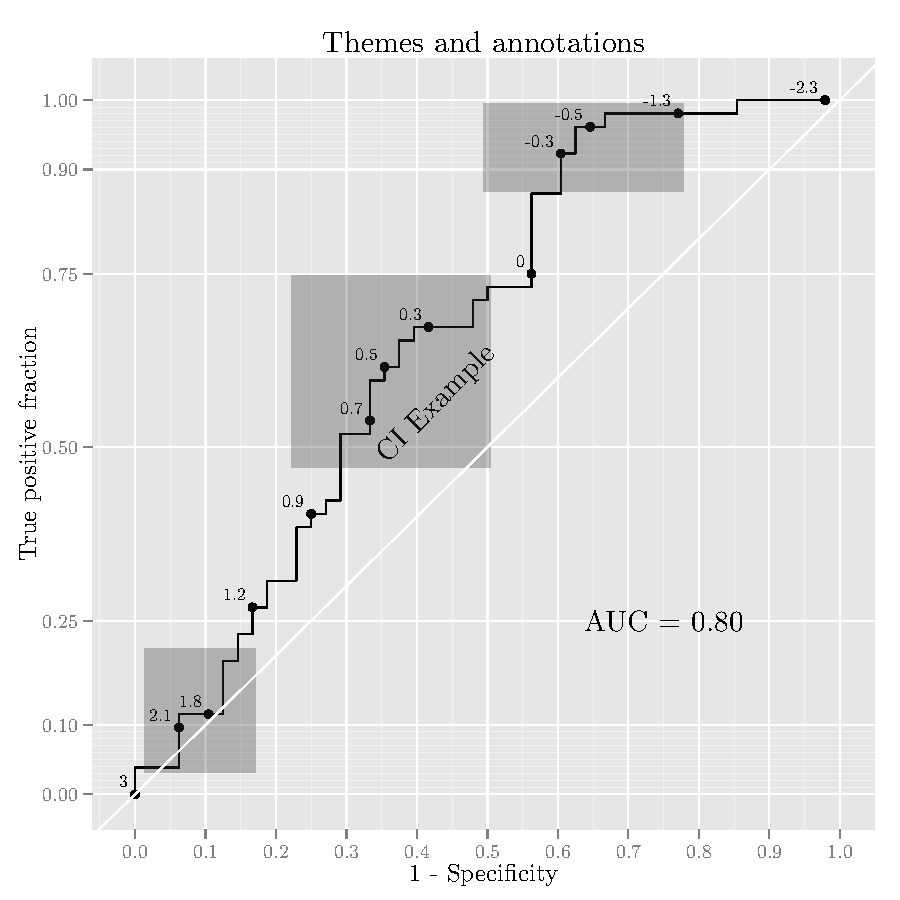
\includegraphics{figure/print2-1.pdf}
\caption{Using \pkg{ggplot2} themes and annotations with \pkg{plotROC}
objects. \label{annotate}}
\end{figure}

\subsubsection{Other estimation methods}\label{other-estimation-methods}

By default \texttt{calculate\_roc} computes the empirical ROC curve.
There are other estimation methods out there, as I have summarized in
the introduction. Any estimation method can be used, as long as the
cutoff, the TPF and the FPF are returned. Then you can simply pass those
values in a data frame to the \texttt{ggroc} function. For example, let
us use the binormal method to create a smooth curve. This approach
assumes that the test distribution is normal conditional on disease
status.

\begin{verbatim}
D.ex <- rbinom(100, 1, .5)
M.ex <- rnorm(100, mean = D.ex, sd = .5)

mu1 <- mean(M.ex[D.ex == 1])
mu0 <- mean(M.ex[D.ex == 0])
s1 <- sd(M.ex[D.ex == 1])
s0 <- sd(M.ex[D.ex == 0])
c.ex <- seq(min(M.ex), max(M.ex), length.out = 300)

binorm.roc <- data.frame(c = c.ex, 
                             FPF = pnorm((mu0 - c.ex)/s0), 
                             TPF = pnorm((mu1 - c.ex)/s1)
                             )
\end{verbatim}

Then I can pass this data.frame to the \texttt{ggroc} function as
before. The example is shown in figure \ref{binorm}.

\begin{verbatim}
binorm.plot <- ggroc(binorm.roc, label = "Binormal")
plot_journal_roc(binorm.plot)
\end{verbatim}

\begin{figure}[htbp]
\centering
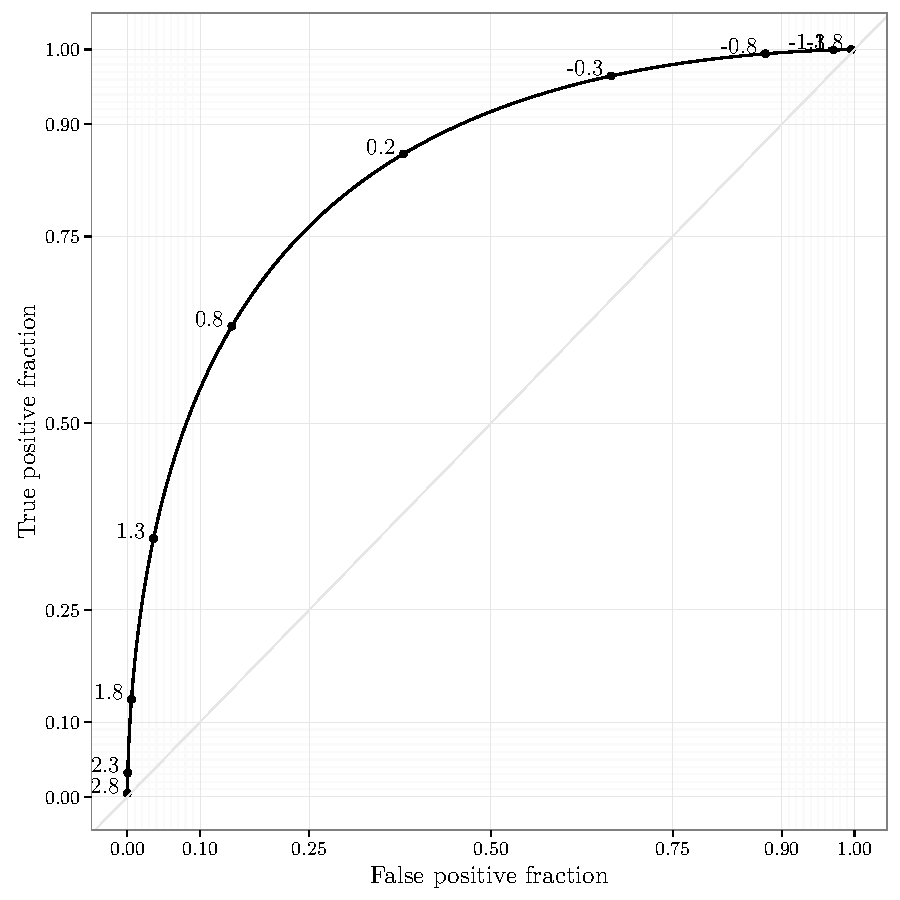
\includegraphics{figure/binormal-1.pdf}
\caption{Illustration of smooth binormal ROC curve. \label{binorm}}
\end{figure}

Another potential use of this approach is for plotting time-dependent
ROC curves for time-to-event outcomes estimated as desribed in
\citep{heagerty2000time}.

\section{How it Works}\label{how-it-works}

\pkg{plotROC} makes use of \pkg{ggplot2} \citep{ggplot2}, \pkg{gridSVG}
\citep{gridsvg}, and \pkg{d3.js} \citep{bostock2011d3} to create
interactive plots. The first step in the process is to create
\texttt{ggplot} objects using the \texttt{ggroc} or
\texttt{multi\_ggroc} functions. These functions return standard
\texttt{ggplot} objects that include basic styling, hidden cutoff
labels, and hidden confidence regions. They can be plotted and inspected
in the \proglang{R} console. These form the basis for both the print
versions and the interactive versions of the plots. Creating a print
version by using the \texttt{plot\_journal\_roc} function simply makes
visible a subset of the hidden cutoff labels and confidence regions, if
available.

\pkg{plotROC} makes interactive plots by first converting the
\texttt{ggplot} object into a scalable vector graphic (svg) object with
the \texttt{grid.export} function. This function maps each element of
the plot to a corresponding element of the svg markup language. I keep
track of the names of the points and labels elements so that I can add
interactivity using \pkg{d3.js} and \proglang{JavaScript}. The main
interactive feature I wanted was to be able to display the cutoff labels
at the points on the ROC curve closest to the mouse cursor.

There are many ways to solve this with \pkg{d3.js}, but I decided to use
Voronoi polygons to map the cursor location to the nearest point on the
ROC curve. The idea is that for the set of cutoff points along the ROC
curve, the \texttt{d3.geom.voronoi} function chain computes a set of
polygons overlaying the plotting region such that the area of each
polygon contains the region of the plot closest to it's corresponding
cutoff point. Hover events are bound to the polygons so that when the
mouse cursor moves around the plotting region, the closest point on the
ROC curve is made visible. Similarly, click events are bound to the
polygons so that the appropriate confidence region is made visible upon
clicking. The svg code and all necessary \proglang{JavaScript} code is
returned in the character string provided by
\texttt{export\_interactive\_roc}. Figure \ref{flow} outlines the
\pkg{plotROC} process.

\begin{figure}[ht]
\centering
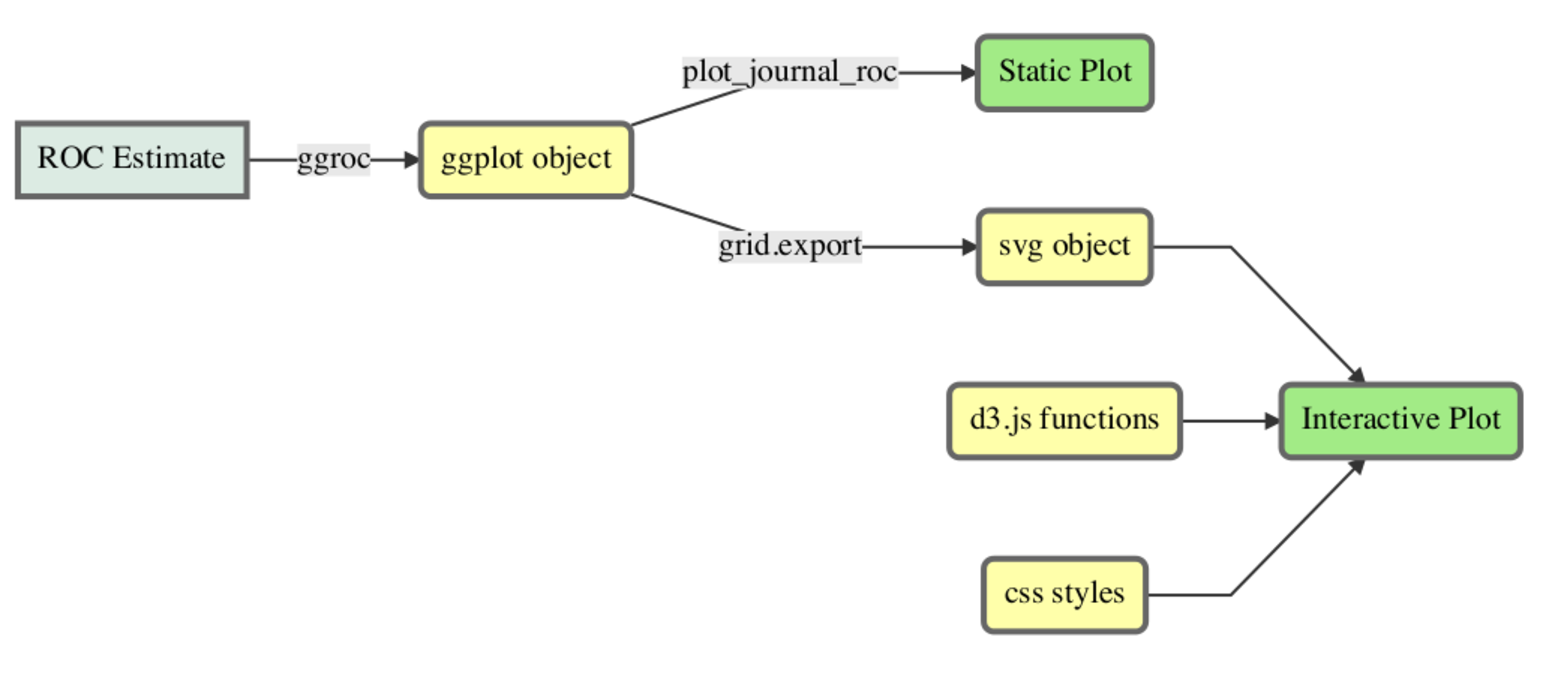
\includegraphics{figure/diagram.pdf}
\caption{Flowchart illustrating the approach that \pkg{plotROC} takes to generate either static plots for print or interactive plots for web-use. \label{flow}}
\end{figure}

This approach is similar to what is done in the \pkg{gridSVG}
\texttt{grid.animate} function, which uses the svg
\texttt{\textless{}animate /\textgreater{}} tags. However, the available
features were not sufficient for my needs, which is why I used
\pkg{d3.js}. There are several other \proglang{R} packages that aim to
create interactive figures. The authors of \pkg{animint} \citep{animint}
created an extensive \proglang{JavaScript} library that creates plots in
a similar way as \pkg{ggplot2}. A set of interactive features can be
added to plots using \pkg{d3.js}. \pkg{ggvis} \citep{ggvis},
\pkg{rCharts} \citep{rcharts}, and the more recently released
\pkg{htmlwidgets} \citep{htmlwidgets} all leverage existing charting
libraries written in \proglang{JavaScript}. Their general approach is to
manipulate the data and create options in \proglang{R}, and then let the
charting libraries handle the rendering and interactivity. \pkg{plotROC}
lets \proglang{R} do the rendering, allowing the figures to be
consistent across print and web-based media, and retaining the
distinctive \proglang{R} style.

\section{Discussion}\label{discussion}

Here I have illustrated the usage and described the mechanics of a new
\proglang{R} package for creating ROC curve plots. The functions are
easy to use, even for non-\proglang{R} users \emph{via} the web
application, yet have sufficient flexibility to meet the needs of power
users. My approach to creating interactive plots differs from other
interactive charting packages. I found that existing approaches did not
meet the highly specialized needs of plotting ROC curves. While ROC
curve plots can technically be created with even the most basic plotting
tools, I find that specialized functions make the results clearer and
more informative.


%\bibliographystyle{jss}
\bibliography{plotroc}


\end{document}
